\documentclass[12pt,letterpaper]{article}\usepackage[]{graphicx}\usepackage[]{color}
%% maxwidth is the original width if it is less than linewidth
%% otherwise use linewidth (to make sure the graphics do not exceed the margin)
\makeatletter
\def\maxwidth{ %
  \ifdim\Gin@nat@width>\linewidth
    \linewidth
  \else
    \Gin@nat@width
  \fi
}
\makeatother

\definecolor{fgcolor}{rgb}{0.345, 0.345, 0.345}
\newcommand{\hlnum}[1]{\textcolor[rgb]{0.686,0.059,0.569}{#1}}%
\newcommand{\hlstr}[1]{\textcolor[rgb]{0.192,0.494,0.8}{#1}}%
\newcommand{\hlcom}[1]{\textcolor[rgb]{0.678,0.584,0.686}{\textit{#1}}}%
\newcommand{\hlopt}[1]{\textcolor[rgb]{0,0,0}{#1}}%
\newcommand{\hlstd}[1]{\textcolor[rgb]{0.345,0.345,0.345}{#1}}%
\newcommand{\hlkwa}[1]{\textcolor[rgb]{0.161,0.373,0.58}{\textbf{#1}}}%
\newcommand{\hlkwb}[1]{\textcolor[rgb]{0.69,0.353,0.396}{#1}}%
\newcommand{\hlkwc}[1]{\textcolor[rgb]{0.333,0.667,0.333}{#1}}%
\newcommand{\hlkwd}[1]{\textcolor[rgb]{0.737,0.353,0.396}{\textbf{#1}}}%

\usepackage{framed}
\makeatletter
\newenvironment{kframe}{%
 \def\at@end@of@kframe{}%
 \ifinner\ifhmode%
  \def\at@end@of@kframe{\end{minipage}}%
  \begin{minipage}{\columnwidth}%
 \fi\fi%
 \def\FrameCommand##1{\hskip\@totalleftmargin \hskip-\fboxsep
 \colorbox{shadecolor}{##1}\hskip-\fboxsep
     % There is no \\@totalrightmargin, so:
     \hskip-\linewidth \hskip-\@totalleftmargin \hskip\columnwidth}%
 \MakeFramed {\advance\hsize-\width
   \@totalleftmargin\z@ \linewidth\hsize
   \@setminipage}}%
 {\par\unskip\endMakeFramed%
 \at@end@of@kframe}
\makeatother

\definecolor{shadecolor}{rgb}{.97, .97, .97}
\definecolor{messagecolor}{rgb}{0, 0, 0}
\definecolor{warningcolor}{rgb}{1, 0, 1}
\definecolor{errorcolor}{rgb}{1, 0, 0}
\newenvironment{knitrout}{}{} % an empty environment to be redefined in TeX

\usepackage{alltt}
\usepackage[left=2cm,right=2cm,top=2cm,bottom=2cm]{geometry}
\usepackage[ansinew]{inputenc}
\usepackage[spanish]{babel}
\usepackage{amsmath}
\usepackage{amsfonts}
\usepackage{amssymb}
\usepackage{dsfont}
\usepackage{multicol} 
\usepackage{subfigure}
\usepackage{graphicx}
\usepackage{float} 
\usepackage{verbatim} 
\usepackage[left=2cm,right=2cm,top=2cm,bottom=2cm]{geometry}
\usepackage{fancyhdr}
\pagestyle{fancy} 
\fancyhead[LO]{\leftmark}
\usepackage{caption}
\newtheorem{definicion}{Definci\'On}
\IfFileExists{upquote.sty}{\usepackage{upquote}}{}
\begin{document}

\begin{titlepage}
\setlength{\unitlength}{1 cm} %Especificar unidad de trabajo

\begin{center}
\textbf{{\large UNIVERSIDAD DE EL SALVADOR}\\
{\large FACULTAD MULTIDISCIPLINARIA DE OCCIDENTE}\\
{\large DEPARTAMENTO DE MATEM\'ATICA}}\\ [0.50 cm]

\begin{picture}(18,4)
 \put(7,0){
\includegraphics[width=4cm]{minerva.jpg}}
\end{picture}
\\[0.25 cm]

\textbf{{\large Licenciatura en Estad\'istica}\\ [1.25cm]
{\large Control Estad\'istico del Paquete R }\\ [2 cm]
%\setlength{\unitlength}{1 cm}
{\large  \textbf{''UNIDAD TRES"}}\\ [3 cm]
{\large Alumna:}\\
{\large Erika Beatr\'iz Guill\'en Pineda}\\ [2cm]
{\large Fecha de elaboraci\'on}\\
Santa Ana - \today }
\end{center}
\end{titlepage}

\newtheorem{teorema}{Teorema}
\newtheorem{prop}{Proposici\'on}[section]

\lhead{Pr\'actica 09}

\lfoot{LICENCIATURA EN ESTAD\'ISTICA}
\cfoot{UESOCC}
\rfoot{\thepage}
%\pagestyle{fancy} 

\setcounter{page}{1}
\newpage

\section {AN\'ALISIS DE UNA VARIABLE BIDIMENSIONAL CATEG\'ORICA}
\textbf{Ejemplo 1:}Se selecciona aleatoriamente una muestra de 18 personas adultas, para estudiar si existe relaci\'on entre su estado civil y su ocupaci\'on.

\subsection{REALICE UN AN\'ALISIS ESTAD?STICO DE LOS DATOS.} 

\textbf{1) Activa tu directorio de trabajo.} 
\begin{knitrout}
\definecolor{shadecolor}{rgb}{0.969, 0.969, 0.969}\color{fgcolor}\begin{kframe}
\begin{alltt}
\hlkwd{getwd}\hlstd{()}
\end{alltt}
\begin{verbatim}
## [1] "C:/Users/User/Documents/TODAS_PRACTICAS"
\end{verbatim}
\begin{alltt}
\hlkwd{setwd}\hlstd{(}\hlstr{"C:/Users/User/Documents/TODAS_PRACTICAS"}\hlstd{)}
\end{alltt}
\end{kframe}
\end{knitrout}
@
\textbf{2) Limpia de objetos el \'area de trabajo (Workspace).} 
\begin{knitrout}
\definecolor{shadecolor}{rgb}{0.969, 0.969, 0.969}\color{fgcolor}\begin{kframe}
\begin{alltt}
\hlkwd{ls}\hlstd{()}
\end{alltt}
\begin{verbatim}
## character(0)
\end{verbatim}
\begin{alltt}
\hlkwd{rm}\hlstd{(}\hlkwc{list}\hlstd{=}\hlkwd{ls}\hlstd{(}\hlkwc{all}\hlstd{=}\hlnum{TRUE}\hlstd{))}
\hlkwd{ls}\hlstd{()}
\end{alltt}
\begin{verbatim}
## character(0)
\end{verbatim}
\end{kframe}
\end{knitrout}
\textbf{3) Crea un nuevo Script y ll?male "Script09-DatosBivariados1".}

\textbf{4) Crea en Excel una hoja de datos con dos columnas o variables} 
\begin{knitrout}
\definecolor{shadecolor}{rgb}{0.969, 0.969, 0.969}\color{fgcolor}\begin{kframe}
\begin{alltt}
\hlcom{# Recuerda que al guardar la hoja, el tipo de archivo es de extensi?n .csv(delimitado por comas).}
\hlcom{# Ll\textbackslash{}'amale al archivo: HojaCat}
\hlcom{# Otra forma de crear la hoja de datos es la siguiente (Vea la Pr?ctica 04):}
\hlcom{# Primero crear las dos variables categ\textbackslash{}'oricas en un editor de texto como NotePad o WordPad,colocando nombre a cada columna, y llam\textbackslash{}'andole "HojaCat.txt".}
\hlcom{# Luego puede leer o recuperar este archivo con la funci\textbackslash{}'on read.table()}
\hlstd{HojaCat} \hlkwb{<-} \hlkwd{read.table}\hlstd{(}\hlstr{"HojaCat.txt"}\hlstd{,} \hlkwc{header}\hlstd{=}\hlnum{TRUE}\hlstd{)}
\hlstd{HojaCat}
\end{alltt}
\begin{verbatim}
##        ESTADO  OCUPACIÓN
## 1      Casado Desocupado
## 2     Soltero    Estudia
## 3     Soltero    Trabaja
## 4      Casado    Estudia
## 5  Acompañado    Trabaja
## 6     Soltero Desocupado
## 7      Casado    Trabaja
## 8      Casado    Estudia
## 9  Acompañado Desocupado
## 10 Acompañado    Estudia
## 11     Casado    Trabaja
## 12    Soltero    Estudia
## 13 Acompañado Desocupado
## 14     Casado Desocupado
## 15    Soltero    Estudia
## 16    Soltero    Trabaja
## 17     Casado Desocupado
## 18    Soltero    Trabaja
\end{verbatim}
\end{kframe}
\end{knitrout}
\textbf{5) Recupera desde el entorno de R la hoja de datos de Excel.} 
\begin{knitrout}
\definecolor{shadecolor}{rgb}{0.969, 0.969, 0.969}\color{fgcolor}\begin{kframe}
\begin{alltt}
\hlstd{HojaCat} \hlkwb{<-} \hlkwd{read.csv}\hlstd{(}\hlstr{"HojaCat.csv"}\hlstd{,} \hlkwc{strip.white}\hlstd{=}\hlnum{TRUE}\hlstd{);}
\hlstd{HojaCat}
\end{alltt}
\begin{verbatim}
##        ESTADO  OCUPACIÓN
## 1      Casado Desocupado
## 2     Soltero    Estudia
## 3     Soltero    Trabaja
## 4      Casado    Estudia
## 5  Acompañado    Trabaja
## 6     Soltero Desocupado
## 7      Casado    Trabaja
## 8      Casado    Estudia
## 9  Acompañado Desocupado
## 10 Acompañado    Estudia
## 11     Casado    Trabaja
## 12    Soltero    Estudia
## 13 Acompañado Desocupado
## 14     Casado Desocupado
## 15    Soltero    Estudia
## 16    Soltero    Trabaja
## 17     Casado Desocupado
## 18    Soltero    Trabaja
\end{verbatim}
\end{kframe}
\end{knitrout}
\textbf{6) Conecta la hoja de datos a la segunda ruta o lista de b?squeda.} 
\begin{knitrout}
\definecolor{shadecolor}{rgb}{0.969, 0.969, 0.969}\color{fgcolor}\begin{kframe}
\begin{alltt}
\hlkwd{attach}\hlstd{(HojaCat,} \hlkwc{pos}\hlstd{=}\hlnum{2}\hlstd{)} \hlcom{# pos especifica la posici\textbackslash{}'on donde buscar la conexi\textbackslash{}'on}
\hlkwd{search}\hlstd{()}
\end{alltt}
\begin{verbatim}
##  [1] ".GlobalEnv"        "HojaCat"           "package:knitr"    
##  [4] "package:stats"     "package:graphics"  "package:grDevices"
##  [7] "package:utils"     "package:datasets"  "package:methods"  
## [10] "Autoloads"         "package:base"
\end{verbatim}
\end{kframe}
\end{knitrout}
\textbf{7) Crea una tabla de contigencia o de doble entrada} 
\begin{knitrout}
\definecolor{shadecolor}{rgb}{0.969, 0.969, 0.969}\color{fgcolor}\begin{kframe}
\begin{alltt}
\hlstd{tablaCont} \hlkwb{<-} \hlkwd{table}\hlstd{(HojaCat);}
\hlstd{tablaCont}
\end{alltt}
\begin{verbatim}
##             OCUPACIÓN
## ESTADO       Desocupado Estudia Trabaja
##   Acompañado          2       1       1
##   Casado              3       2       2
##   Soltero             1       3       3
\end{verbatim}
\begin{alltt}
\hlkwd{length}\hlstd{(HojaCat)}
\end{alltt}
\begin{verbatim}
## [1] 2
\end{verbatim}
\begin{alltt}
\hlcom{# sino m\textbackslash{}'as bien el n\textbackslash{}'umero de variables o columnas consideradas }
\hlcom{# en el conjunto de datos.}

\hlcom{# Encuentra la suma de cada fila de la tabla de contingencia}
\hlcom{# Distribuci\textbackslash{}'on marginal de X=Estado civil}
\hlstd{suma.filas} \hlkwb{<-} \hlkwd{apply}\hlstd{(tablaCont,} \hlnum{1}\hlstd{, sum);}
\hlstd{suma.filas}
\end{alltt}
\begin{verbatim}
## Acompañado     Casado    Soltero 
##          4          7          7
\end{verbatim}
\begin{alltt}
\hlcom{# El 1 indica que son totales por fila}
\hlcom{# Encuentra la suma de cada fila de la tabla de contingencia}
\hlcom{# distribuci\textbackslash{}'on marginal de Y=Ocupaci\textbackslash{}'on}

\hlstd{suma.columnas} \hlkwb{<-} \hlkwd{apply}\hlstd{(tablaCont,}\hlnum{2}\hlstd{,sum);}
\hlstd{suma.columnas}
\end{alltt}
\begin{verbatim}
## Desocupado    Estudia    Trabaja 
##          6          6          6
\end{verbatim}
\begin{alltt}
\hlcom{# 2 indica que son totales por columna}
\hlcom{# Gr\textbackslash{}'aficos de barras para tabla de contingencia.}
\hlcom{# Barras apiladas}

\hlkwd{barplot}\hlstd{(}\hlkwd{t}\hlstd{(tablaCont),} \hlkwc{main}\hlstd{=}\hlstr{"Grafico de barras (Estado, Ocupacion)"}\hlstd{,}
        \hlkwc{xlab}\hlstd{=}\hlstr{"Estado civil"}\hlstd{,}
\hlkwc{ylab}\hlstd{=}\hlstr{"Ocupacion"}\hlstd{,} \hlkwc{legend.text}\hlstd{=}\hlnum{TRUE}\hlstd{)}
\end{alltt}
\end{kframe}
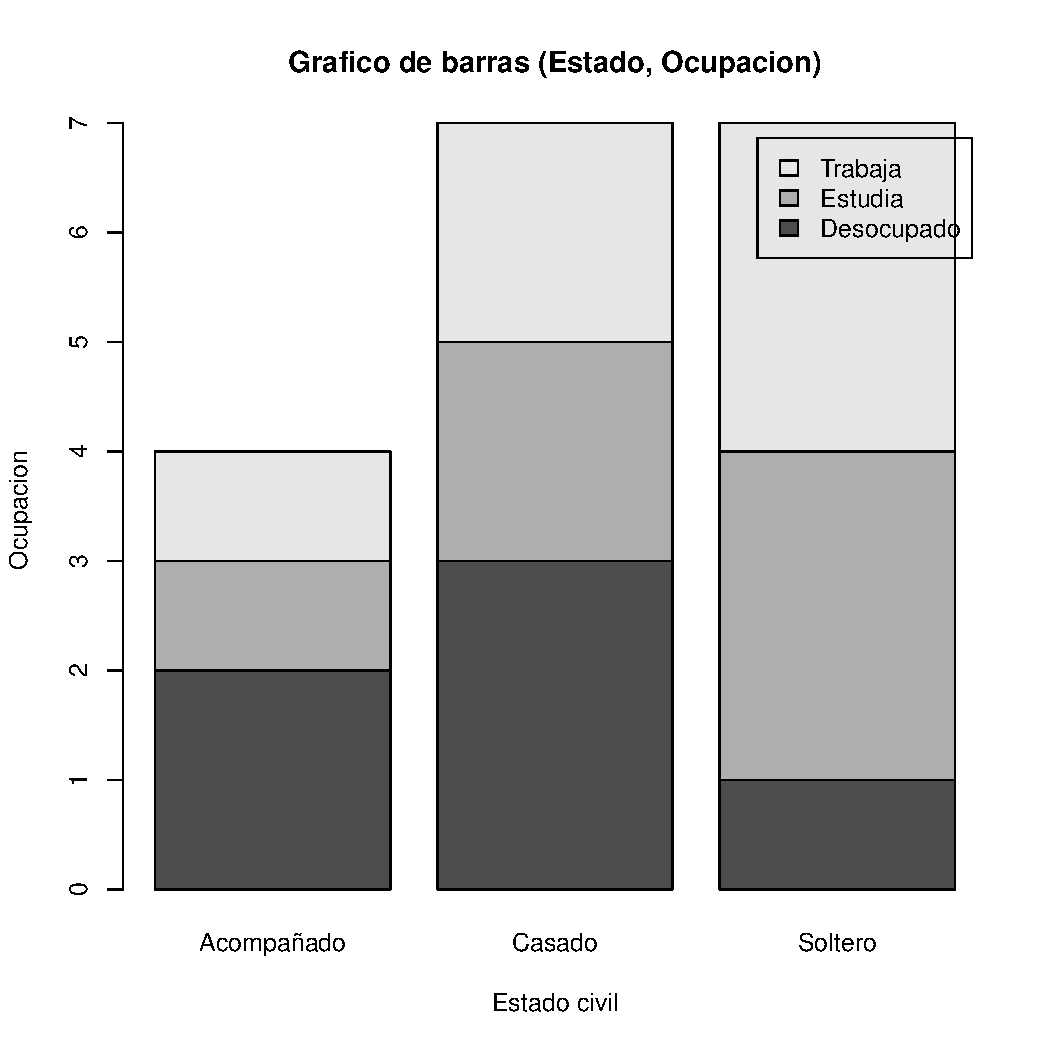
\includegraphics[width=\maxwidth]{figure/unnamed-chunk-6-1} 
\begin{kframe}\begin{alltt}
\hlcom{# Note que t(tablaCont) indica que las barras representan el }
\hlcom{# Estado civil de los encuestados y que \textbackslash{}'estas se subdividen en }
\hlcom{# cada una de las diferentes ocupaciones consideradas.}
\hlcom{# En caso de usar \textbackslash{}'unicamente tablaCont; las barras representar\textbackslash{}'on }
\hlcom{# las diferentes ocupaciones y ?stas estar\textbackslash{}'an subdividas en cada uno }
\hlcom{# de los estados civiles.}

\hlcom{# Barras agrupadas}
\hlkwd{barplot}\hlstd{(}\hlkwd{t}\hlstd{(tablaCont),} \hlkwc{main}\hlstd{=}\hlstr{"Grafico de barras (Estado, Ocupacion)"}\hlstd{,}
        \hlkwc{xlab}\hlstd{=}\hlstr{"Estado civil"}\hlstd{,} \hlkwc{ylab}\hlstd{=}\hlstr{"Ocupacion"}\hlstd{,} \hlkwc{beside}\hlstd{=}\hlnum{TRUE}\hlstd{,} \hlkwc{legend.text}\hlstd{=}\hlnum{TRUE}\hlstd{)}
\end{alltt}
\end{kframe}
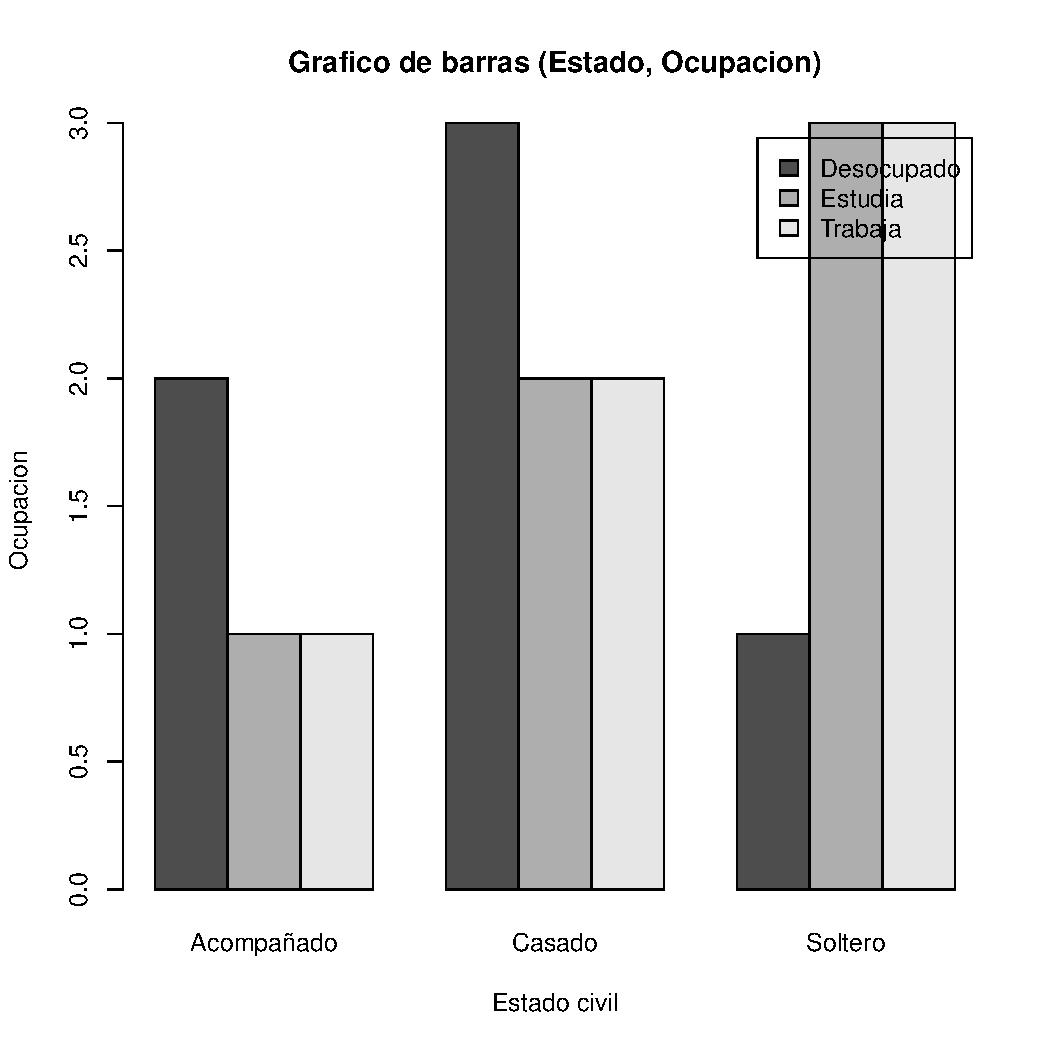
\includegraphics[width=\maxwidth]{figure/unnamed-chunk-6-2} 
\begin{kframe}\begin{alltt}
\hlcom{# Note que la instrucci\textbackslash{}'on beside =TRUE, indica que por cada una de }
\hlcom{# las diferentes ocupaciones se crear? una barra para cada estado civil. }
\hlcom{# Note que al usar beside =FALSE se obtiene el mismo gr\textbackslash{}'afico de la }
\hlcom{# instrucci\textbackslash{}'on anterior.}

\hlkwd{barplot}\hlstd{(tablaCont,} \hlkwc{main}\hlstd{=}\hlstr{"Grafico de barras (Ocupacion, Estado)"}\hlstd{,}
        \hlkwc{xlab}\hlstd{=}\hlstr{"Ocupacion\textbackslash{}n"}\hlstd{,}
\hlkwc{ylab}\hlstd{=}\hlstr{"Estado civil"}\hlstd{,} \hlkwc{beside}\hlstd{=}\hlnum{TRUE}\hlstd{,} \hlkwc{legend.text}\hlstd{=}\hlnum{TRUE}\hlstd{)}
\end{alltt}
\end{kframe}
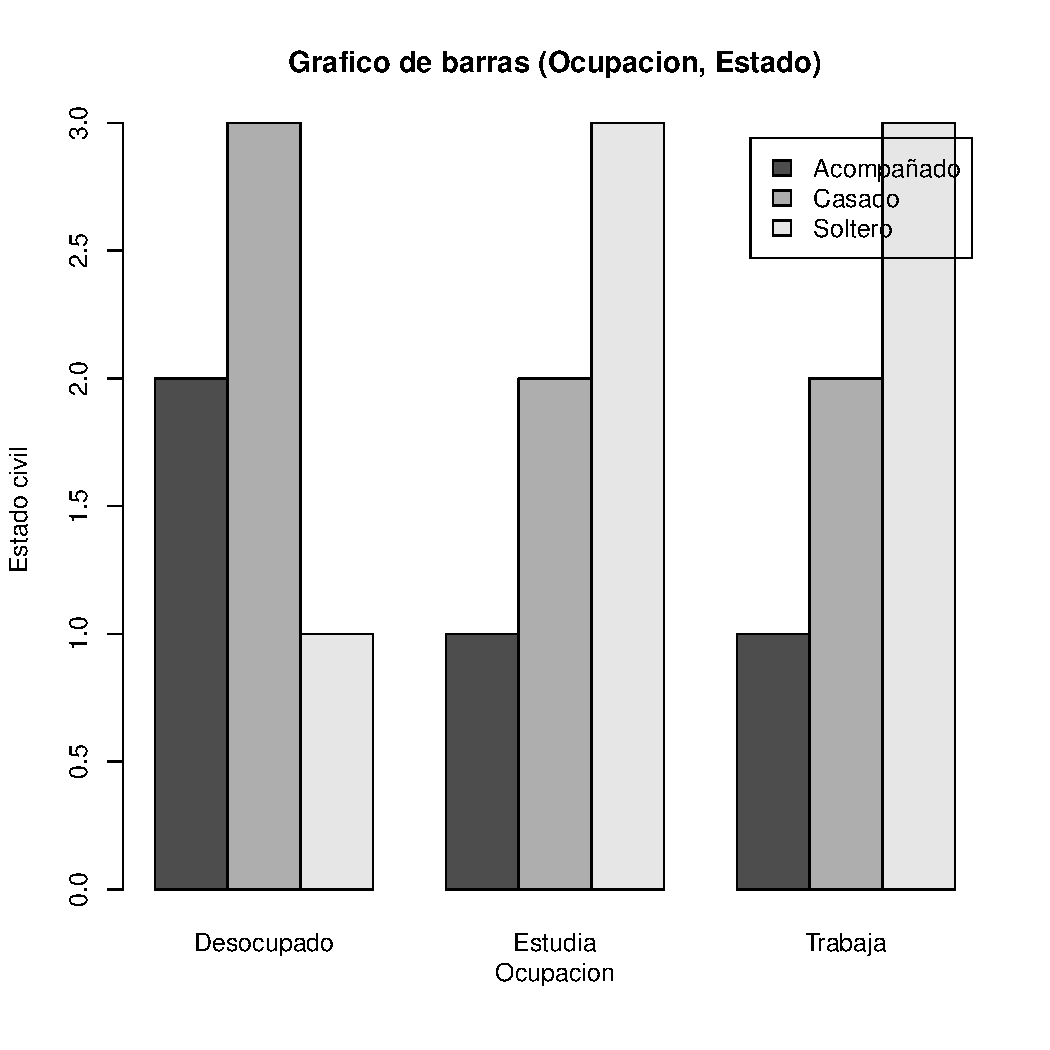
\includegraphics[width=\maxwidth]{figure/unnamed-chunk-6-3} 

\end{knitrout}
\textbf{8) Calcula tablas de proporciones o de probabilidades.} 
\begin{knitrout}
\definecolor{shadecolor}{rgb}{0.969, 0.969, 0.969}\color{fgcolor}\begin{kframe}
\begin{alltt}
\hlstd{op} \hlkwb{<-} \hlkwd{options}\hlstd{()}
\hlkwd{options}\hlstd{(}\hlkwc{digits}\hlstd{=}\hlnum{3}\hlstd{)} \hlcom{# S\textbackslash{}'olo imprime 3 lugares decimales}
\hlkwd{options}\hlstd{(}\hlstr{'digits'}\hlstd{)}
\end{alltt}
\begin{verbatim}
## $digits
## [1] 3
\end{verbatim}
\begin{alltt}
\hlcom{# Proporciones basadas en el total de la muestra, la suma de filas }
\hlcom{# y columnas suman 1.}
\hlstd{propTotal} \hlkwb{<-} \hlkwd{prop.table}\hlstd{(tablaCont); propTotal}
\end{alltt}
\begin{verbatim}
##             OCUPACIÓN
## ESTADO       Desocupado Estudia Trabaja
##   Acompañado     0.1111  0.0556  0.0556
##   Casado         0.1667  0.1111  0.1111
##   Soltero        0.0556  0.1667  0.1667
\end{verbatim}
\begin{alltt}
\hlkwd{barplot}\hlstd{(}\hlkwd{t}\hlstd{(propTotal),} \hlkwc{main}\hlstd{=}\hlstr{"Grafico de barras (Estado, Ocupacion)"}\hlstd{,}
        \hlkwc{xlab}\hlstd{=}\hlstr{"Estado civil\textbackslash{}n"}\hlstd{,}
\hlkwc{ylab}\hlstd{=}\hlstr{"Ocupacion"}\hlstd{,} \hlkwc{beside}\hlstd{=}\hlnum{TRUE}\hlstd{,} \hlkwc{legend.text}\hlstd{=}\hlnum{TRUE}\hlstd{)}
\end{alltt}
\end{kframe}
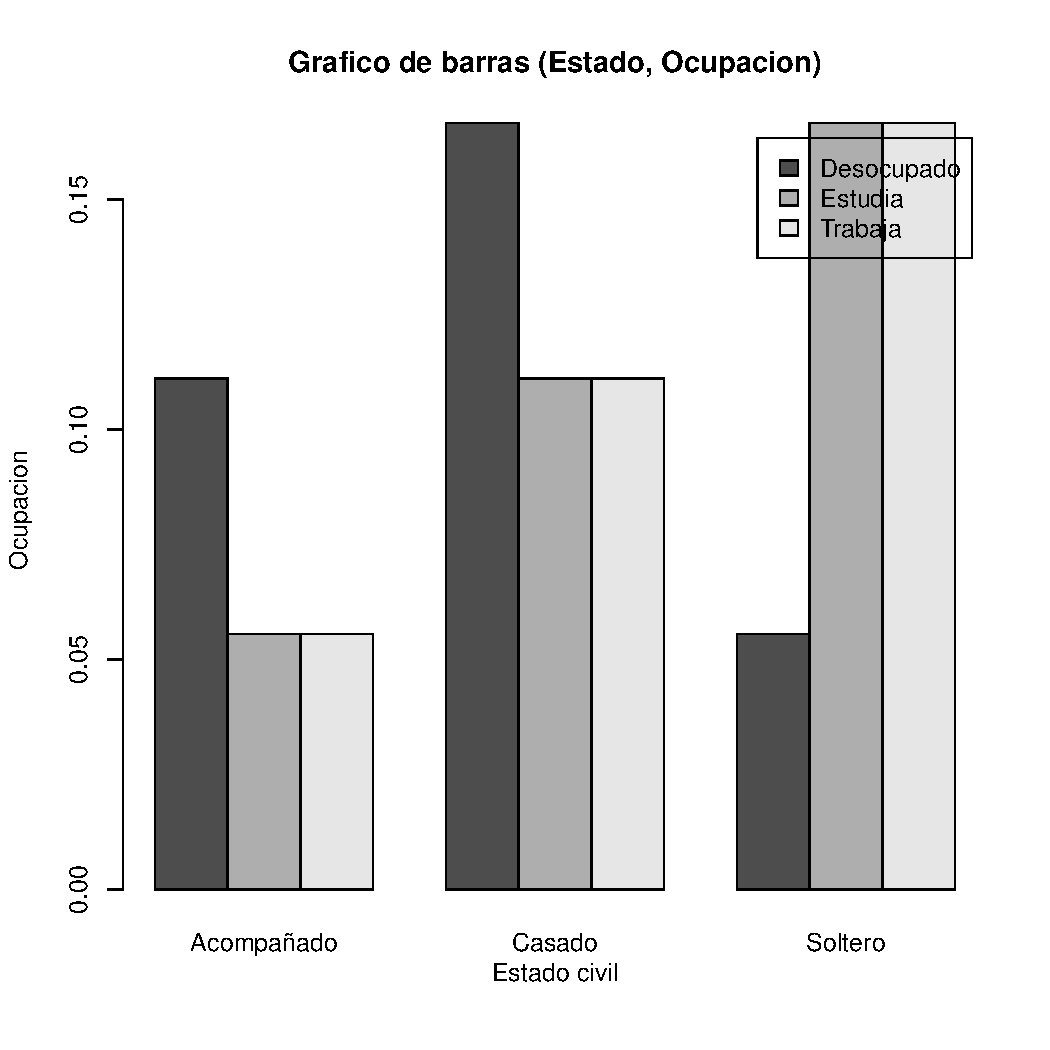
\includegraphics[width=\maxwidth]{figure/unnamed-chunk-7-1} 
\begin{kframe}\begin{alltt}
\hlcom{# Proporciones basadas en el total por fila, cada fila suma 1.}
\hlstd{propFila} \hlkwb{<-} \hlkwd{prop.table}\hlstd{(tablaCont,} \hlnum{1}\hlstd{);}
\hlstd{propFila}
\end{alltt}
\begin{verbatim}
##             OCUPACIÓN
## ESTADO       Desocupado Estudia Trabaja
##   Acompañado      0.500   0.250   0.250
##   Casado          0.429   0.286   0.286
##   Soltero         0.143   0.429   0.429
\end{verbatim}
\begin{alltt}
\hlcom{# Total por fila se indica en 1}
\hlkwd{barplot}\hlstd{(}\hlkwd{t}\hlstd{(propFila),} \hlkwc{main}\hlstd{=}\hlstr{"Grafico de barras (Estado, Ocupacion)"}\hlstd{,}
        \hlkwc{xlab}\hlstd{=}\hlstr{"Estado civil\textbackslash{}n"}\hlstd{,}
\hlkwc{ylab}\hlstd{=}\hlstr{"Ocupacion"}\hlstd{,} \hlkwc{beside}\hlstd{=}\hlnum{TRUE}\hlstd{,} \hlkwc{legend.text}\hlstd{=}\hlnum{TRUE}\hlstd{)}
\end{alltt}
\end{kframe}
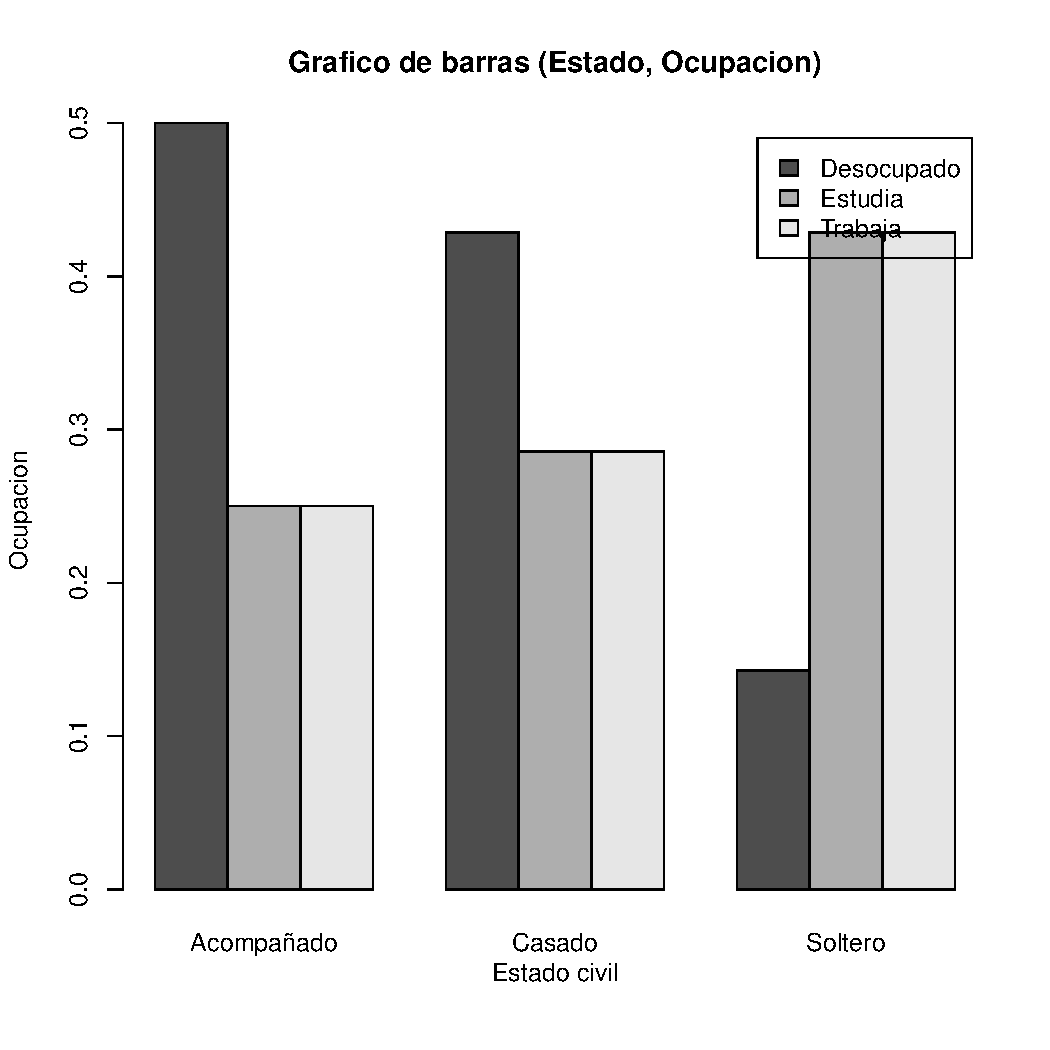
\includegraphics[width=\maxwidth]{figure/unnamed-chunk-7-2} 
\begin{kframe}\begin{alltt}
\hlcom{# Proporciones basadas en el total por columna, cada columna suma 1.}
\hlstd{propColum} \hlkwb{<-} \hlkwd{prop.table}\hlstd{(tablaCont,} \hlnum{2}\hlstd{);}
\hlstd{propColum}
\end{alltt}
\begin{verbatim}
##             OCUPACIÓN
## ESTADO       Desocupado Estudia Trabaja
##   Acompañado      0.333   0.167   0.167
##   Casado          0.500   0.333   0.333
##   Soltero         0.167   0.500   0.500
\end{verbatim}
\begin{alltt}
\hlcom{# Total por columna se indica en 2}
\hlkwd{barplot}\hlstd{(propColum,} \hlkwc{main}\hlstd{=}\hlstr{"Grafico de barras (Ocupacion, Estado)"}\hlstd{,}
        \hlkwc{xlab}\hlstd{=}\hlstr{"Ocupacion\textbackslash{}n"}\hlstd{,}
\hlkwc{ylab}\hlstd{=}\hlstr{"Estado civil"}\hlstd{,} \hlkwc{beside}\hlstd{=}\hlnum{TRUE}\hlstd{,} \hlkwc{legend.text}\hlstd{=}\hlnum{TRUE}\hlstd{)}
\end{alltt}
\end{kframe}
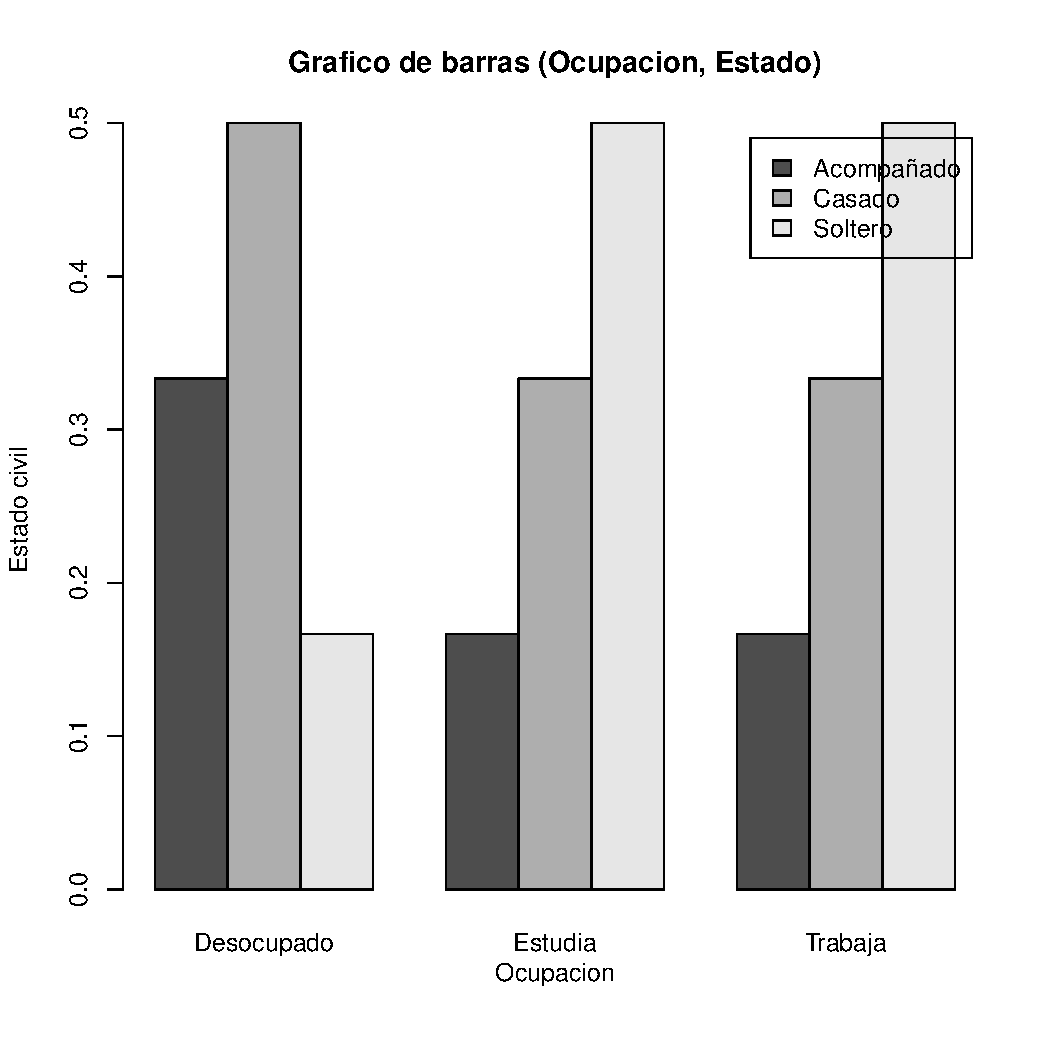
\includegraphics[width=\maxwidth]{figure/unnamed-chunk-7-3} 

\end{knitrout}
\textbf{9) Otra forma de elaborar los gr\'aficos de barras para el vector bidimensional categ?rico.} 
\begin{knitrout}
\definecolor{shadecolor}{rgb}{0.969, 0.969, 0.969}\color{fgcolor}\begin{kframe}
\begin{alltt}
\hlcom{# Gr\textbackslash{}'afico de barras no apiladas y colocaci\textbackslash{}'on de leyenda}
\hlkwd{barplot}\hlstd{(}\hlkwd{table}\hlstd{(Ocupacion, Estado),} \hlkwc{main}\hlstd{=}\hlstr{"Grafico de barras (Estado, Ocupacion)"}\hlstd{,}
        \hlkwc{xlab} \hlstd{=}\hlstr{"Estado Civil"}\hlstd{,} \hlkwc{ylab}\hlstd{=}\hlstr{"Ocupacion"}\hlstd{,} \hlkwc{beside}\hlstd{=}\hlnum{TRUE}\hlstd{,} \hlkwc{legend.text}\hlstd{=}\hlnum{TRUE}\hlstd{)}
\end{alltt}


{\ttfamily\noindent\bfseries\color{errorcolor}{\#\# Error in table(Ocupacion, Estado): objeto 'Ocupacion' no encontrado}}\begin{alltt}
\hlkwd{barplot}\hlstd{(}\hlkwd{table}\hlstd{(Estado, Ocupacion),} \hlkwc{main}\hlstd{=}\hlstr{"Grafico de barras (Ocupacion, Estado)"}\hlstd{,}
        \hlkwc{xlab}\hlstd{=}\hlstr{"Ocupacion"}\hlstd{,} \hlkwc{ylab}\hlstd{=}\hlstr{"Estado civil"}\hlstd{,} \hlkwc{beside}\hlstd{=}\hlnum{TRUE}\hlstd{,} \hlkwc{legend.text}\hlstd{=}\hlnum{TRUE}\hlstd{)}
\end{alltt}


{\ttfamily\noindent\bfseries\color{errorcolor}{\#\# Error in table(Estado, Ocupacion): objeto 'Estado' no encontrado}}\begin{alltt}
\hlkwd{barplot}\hlstd{(}\hlkwd{table}\hlstd{(Estado, Ocupacion),} \hlkwc{main}\hlstd{=}\hlstr{"Grafico de barras (Ocupacion, Estado)"}\hlstd{,}
\hlkwc{xlab}\hlstd{=}\hlstr{"Ocupacion"}\hlstd{,} \hlkwc{ylab}\hlstd{=}\hlstr{"Estado civil"}\hlstd{,} \hlkwc{beside}\hlstd{=}\hlnum{TRUE}\hlstd{,}
\hlkwc{legend.text}\hlstd{=}\hlkwd{c}\hlstd{(}\hlstr{"menor que 2"}\hlstd{,} \hlstr{"2-3"}\hlstd{,}\hlstr{"mayor que 3"}\hlstd{))}
\end{alltt}


{\ttfamily\noindent\bfseries\color{errorcolor}{\#\# Error in table(Estado, Ocupacion): objeto 'Estado' no encontrado}}\begin{alltt}
\hlcom{# Note que se puede definir a conveniencia la leyenda que se desea incorporar }
\hlcom{# en el gr\textbackslash{}'afico con la instrucci\textbackslash{}'on legend.text}
\end{alltt}
\end{kframe}
\end{knitrout}
\textbf{10) Realizar la prueba o contraste Chi-cuadrado de independencia} 
\begin{knitrout}
\definecolor{shadecolor}{rgb}{0.969, 0.969, 0.969}\color{fgcolor}\begin{kframe}
\begin{alltt}
\hlstd{prueba} \hlkwb{<-} \hlkwd{chisq.test}\hlstd{(tablaCont); prueba}
\end{alltt}


{\ttfamily\noindent\color{warningcolor}{\#\# Warning in chisq.test(tablaCont): Chi-squared approximation may be incorrect}}\begin{verbatim}
## 
## 	Pearson's Chi-squared test
## 
## data:  tablaCont
## X-squared = 2, df = 4, p-value = 0.7
\end{verbatim}
\begin{alltt}
\hlcom{# Tenga en cuenta que las frecuencias esperadas deben ser todas mayores a 5}
\hlcom{# Frecuencias absolutas esperadas para la prueba Chi-cuadrada}
\hlstd{prueba}\hlopt{$}\hlstd{expected} \hlcom{# fij = fi./No. column}
\end{alltt}
\begin{verbatim}
##             OCUPACIÓN
## ESTADO       Desocupado Estudia Trabaja
##   Acompañado       1.33    1.33    1.33
##   Casado           2.33    2.33    2.33
##   Soltero          2.33    2.33    2.33
\end{verbatim}
\end{kframe}
\end{knitrout}

\end{document}
